\documentclass[a4paper,11pt,notitlepage]{article}
\usepackage{amsmath}
\usepackage{amsfonts}
\usepackage{amssymb}
\usepackage[UTF8]{ctex}
\usepackage{graphicx}
\usepackage{color}
\usepackage{changepage}
\usepackage{enumitem}
\usepackage{subfigure}
\usepackage{float}
\usepackage[backend=biber]{biblatex}

\usepackage{titlesec}
\titleformat{\section}{\bfseries\Large}{$\S$\,\thesection}{1em}{}
\titleformat{\subsection}{\bfseries\large}{\Roman{subsection}}{1em}{}
\titleformat{\subsubsection}{\bfseries\normalsize}{\roman{subsubsection}}{1em}{}
\titlespacing*{\subsection}{2em}{2pt}{2pt}
\titlespacing*{\subsubsection}{3em}{2pt}{2pt}
\title{\vspace{-1.5cm} \textbf{\huge{数值分析第5章上机}}\vspace{-1em}}
\author{By 211870125 陈睿硕}
\date{}

\usepackage{geometry}
\geometry{left=2cm,right=2cm,top=2cm,bottom=2cm}

\usepackage{fancyhdr}
\pagestyle{fancy}
\fancyhf{}
\fancyhead[L]{Chapter 5}
\fancyhead[R]{\thepage}
\setlength{\headheight}{14pt}

\usepackage{listings}  % 引入 listings 包
\lstset{                % 定义代码块的样式
    basicstyle=\normalsize\ttfamily, % 设定代码字体大小、样式
    showspaces=false,   % 不显示空格
    showstringspaces=false, % 不显示字符串中的空格
    showtabs=false,     % 不显示制表符
    frame=single,       % 设定代码块边框样式
    rulecolor=\color{black}, % 设定代码块边框颜色
    tabsize=4,          % 设定制表符长度为 4 个字符
    captionpos=t,       % 设定标题位置为底部
    keywordstyle=\bfseries\color{blue}\ttfamily,
    stringstyle=\color{red}\ttfamily,
    commentstyle=\color{green}\ttfamily,
    morecomment=[l][\color{magenta}]{\#},
    framesep=0.5em,
    frameround=tttt,
    breaklines=true,    % 自动换行
    breakatwhitespace=false, % 只在空格分割处换行
    escapeinside={\%*}{*)}   % 允许使用 LaTeX 命令
}
\renewcommand{\lstlistingname}{代码}

\usepackage{hyperref}
\usepackage{cleveref}
\crefname{theorem}{定理}{定理}
\crefname{figure}{图}{图}
\crefname{equation}{式}{式}
\crefname{listing}{代码}{代码}

\begin{document}
\maketitle
\vspace{-1cm}
\thispagestyle{fancy}

\section{问题}
\begin{adjustwidth}{1em}{0pt}
\begin{enumerate}[label=\textbf{Q\arabic*}]
    \item 数学上已经证明$\int^{1}_{0}f(x)dx=\pi$,其中$f(x)=\frac{4}{1+x^2}$。分别使用复合梯形,复合 Simpson 求积公式计算
          $\pi$的近似值。选择不同的 h , 对每种求积公式,试将误差刻画成对每种求积公式,试将误差刻画成 h 的函数,
          并比较两方法的精度。是否存在某个 h 值,当低于这个值之后再继续减小 h 的值,计算不再有所改进?为什么?\label{Q1}\notag
    \item 实现 Romberg 求积方法,重复\ref{Q1}的过程。\label{Q2}\notag
    \item 实现 自适应积分方法,重复\ref{Q1}的过程。\label{Q3}\notag
    \item 用等距节点$x_{i}=-5+i,i=0,1,\cdots,10.$给出它的三次自然样条插值函数的图像;\label{Q4}\notag
    \item 用等距节点$x_{i}=-5+i,i=0,1,\cdots,10.$给出它的分段三次Hermite插值函数的图像;\label{Q5}\notag
\end{enumerate}
\end{adjustwidth}

\section{算法思路}
\subsection{对\ref{Q1}的解答}
我们实现了复合梯形,复合 Simpson 求积方法,代码见\cref{code1.1}。得到h和误差(绝对值)的关系如\cref{pic:1}。
\begin{figure}[H]
    \centering
    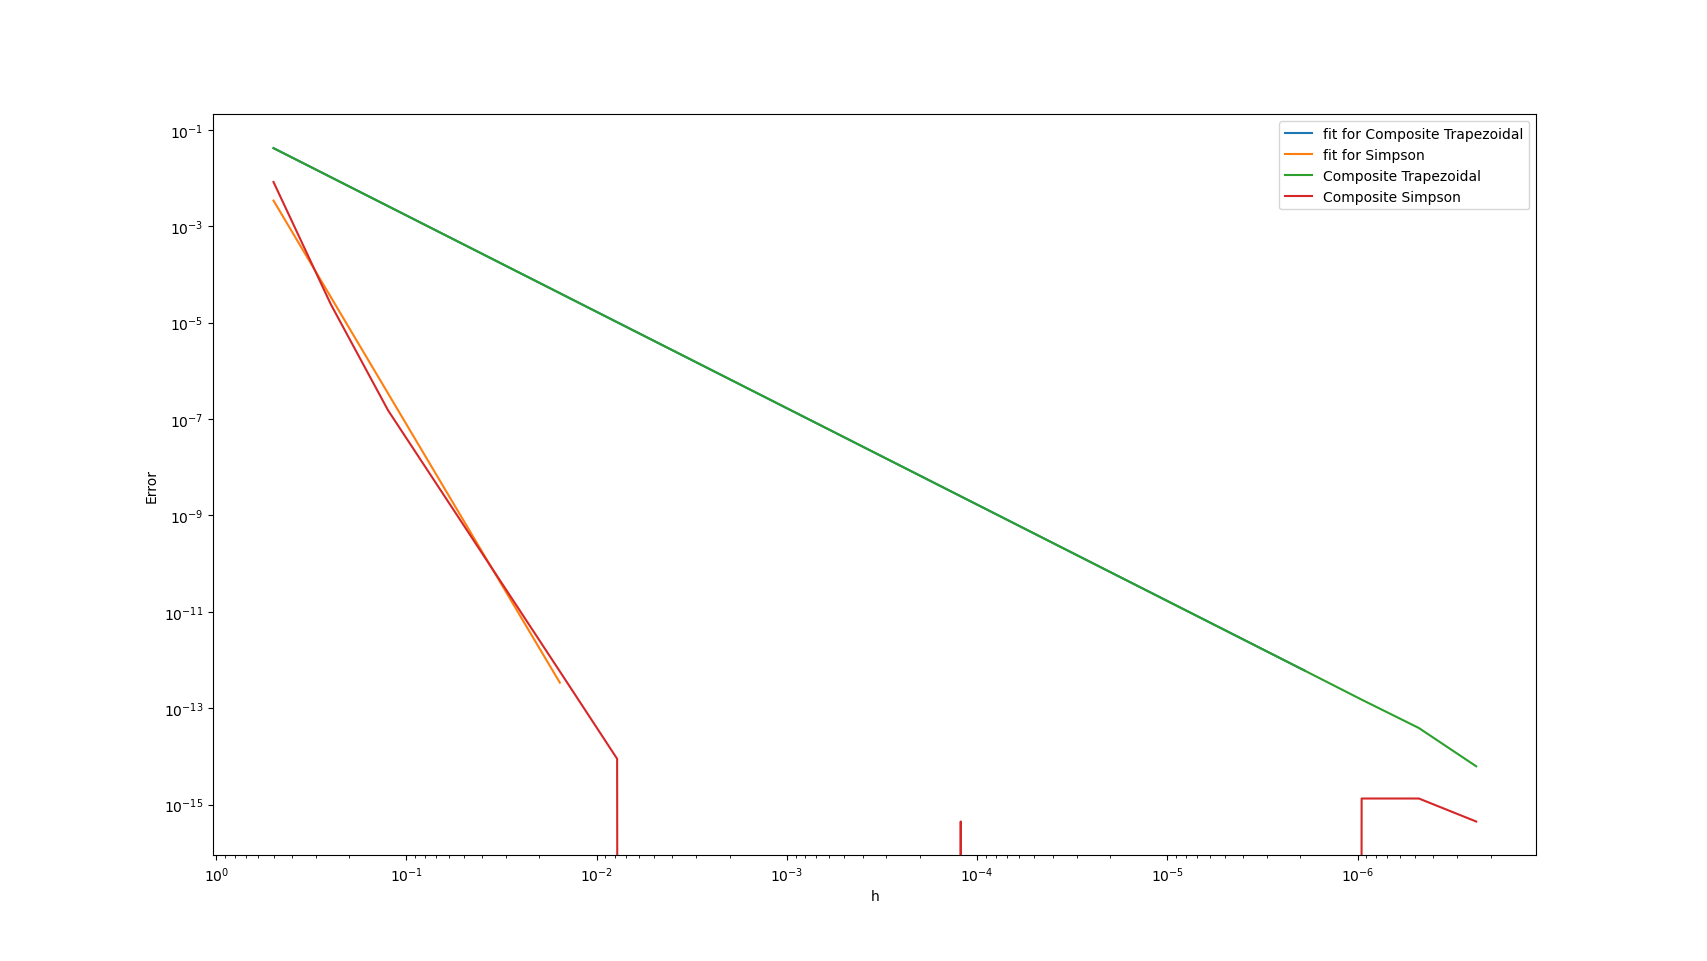
\includegraphics[width=0.8\textwidth]{../picture/Fifth_Chapter_1A.png}
    \caption{10次Newton插值多项式}
    \label{pic:1}
\end{figure}

\subsection{对\ref{Q2}的解答}
使用Python实现,代码见\cref{code2.1}。
如\cref{pic:2}。
\begin{figure}[H]
    \centering
    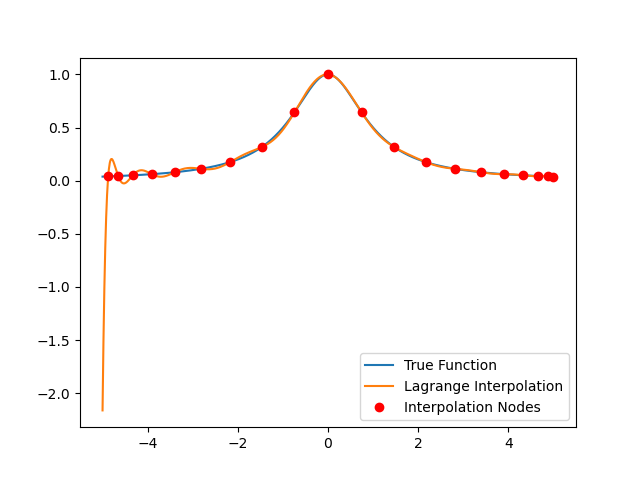
\includegraphics[width=0.8\textwidth]{../picture/Fourth_Week_1B.png}
    \caption{20次Lagrange插值多项式}
    \label{pic:2}
\end{figure}

\subsection{对\ref{Q3}的解答}
使用Python实现,代码见\cref{code3.1}。
如\cref{pic:3}。
\begin{figure}[H]
    \centering
    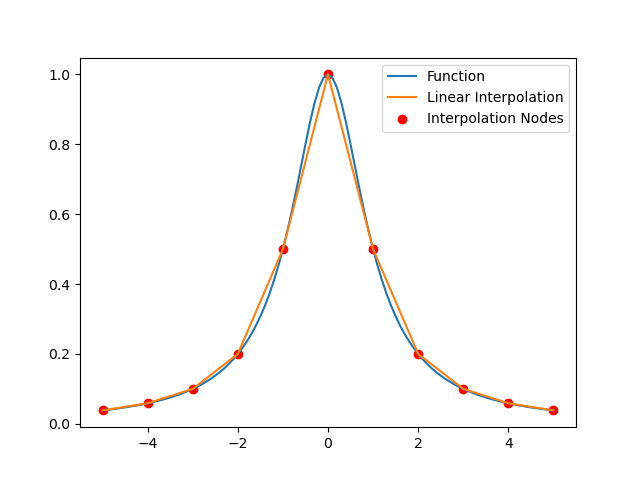
\includegraphics[width=0.8\textwidth]{../picture/Fourth_Week_1C.png}
    \caption{分段线性插值函数}
    \label{pic:3}
\end{figure}

\subsection{对\ref{Q4}的解答}
可以快捷地调用scipy.interpolate中的CubicSpline库完成,见\cref{code4.1}。也可以”从零开始“,
将三次样条插值函数展开,使用Python程序计算其系数,见\cref{code4.2}。
如\cref{pic:4}。
\begin{figure}[H]
    \centering
    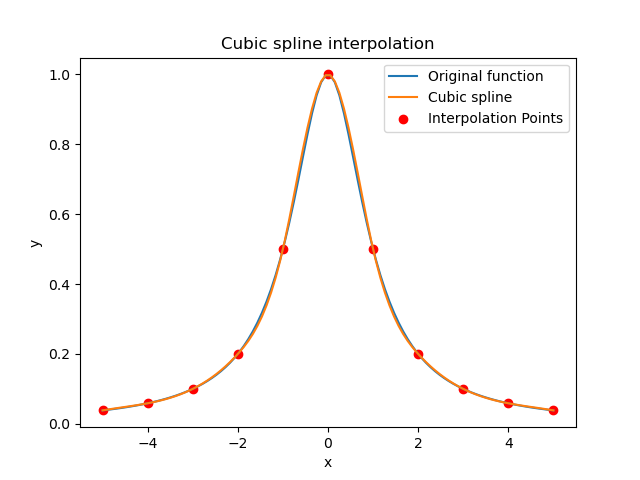
\includegraphics[width=0.8\textwidth]{../picture/Fourth_Week_1D.png}
    \caption{三次自然样条插值函数}
    \label{pic:4}
\end{figure}

\subsection{对\ref{Q5}的解答}
调用scipy.interpolate中的PchipInterpolator库完成,见\cref{code5.1}。也可以”从零开始“。
由于此处是等距插值,故可以手动解出$m_{i},i=1,2,\cdots,n+1$(书上记号),写出系数表达式,从而直接求出每个小区间
的三次Hermite插值多项式。见\cref{code5.2}。
如\cref{pic:5}。
\begin{figure}[H]
    \centering
    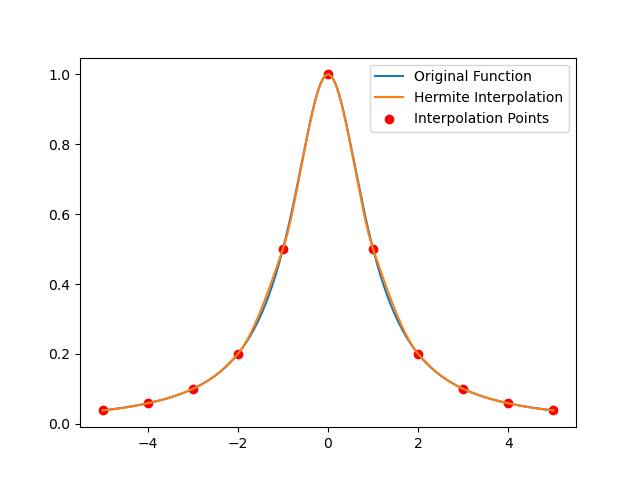
\includegraphics[width=0.8\textwidth]{../picture/Fourth_Week_1E.png}
    \caption{分段三次Hermite插值函数}
    \label{pic:5}
\end{figure}

\section{结果分析}
\subsection{对\ref{Q1}的分析}
可以看到,h和误差的关系在h不特别小时几乎是对数线性关系,对于复合积分法$Error\approx 10^{-0.77821}h^{2.0000}$,
而对于复合Simpson法$Error\approx 10^{-0.46800}h^{6.6460}$。\\
我们知道,复合梯形公式的误差(绝对值)$Error=\frac{1}{12}h^2f''(\xi )$,其中$\xi \in (0,1)$,
这与我们的估计式相吻合($f''(x)$在$[0,1]$上变化不大)。\\
而复合Simpson公式的误差(绝对值)$Error=\frac{1}{180}h^4f''(\xi )$,其中$\xi \in (0,1)$,
这就与我们的估计式有一定的差距,可能是因为拟合的位置h值还比较大。


\subsection{对\ref{Q2}的分析}
观察\cref{pic:2}可知,此时的插值多项式Runge现象并不严重,这主要是因为采用了Chebyshev插值法,导致误差的上界被严格控制,
故函数逼近较为准确。

\subsection{对\ref{Q3}的分析}
观察\cref{pic:3}可知,线性插值函数无Runge现象,但插值函数在插值点处不平滑。

\subsection{对\ref{Q4}、\ref{Q5}的分析}
观察\cref{pic:4}、\cref{pic:5}可知,分段三次Hermite插值函数和分段三次样条差值函数都不会发生Runge现象,
这主要是因为小区间拟合减少了插值函数的可波动性(即减少了与原函数之间的差值上界)。

\section{附录:程序代码}
\begin{lstlisting}[language=Python,caption={Fifth Chapter 1A.py},label={code1.1}]
import numpy as np
import matplotlib.pyplot as plt


def f(x):
    return 4 / (1 + x**2)


def composite_trapezoidal(a, b, h):
    n = int((b - a) / h)
    x = np.linspace(a, b, n+1)
    y = f(x)
    s = (y[0] + y[n] + 2 * np.sum(y[1:n])) * h / 2
    return s


def composite_simpson(a, b, h):
    n = int((b - a) / h)
    x = np.linspace(a, b, n+1)
    y = f(x)
    s = (y[0] + y[n] + 4 * np.sum(y[1:n:2]) + 2 * np.sum(y[2:n-1:2])) * h / 3
    return s


a, b = 0, 1

trap_errors = np.array([])
simp_errors = np.array([])

h_values = np.array([0.5**i for i in range(1, 23)])

for i in h_values:
    trap_error = np.abs(composite_trapezoidal(a, b, i) - np.pi)
    simp_error = np.abs(composite_simpson(a, b, i) - np.pi)
    trap_errors = np.append(trap_errors, trap_error)
    simp_errors = np.append(simp_errors, simp_error)

mask1 = np.where(h_values > 1e-6)
coefficients1 = np.polyfit(
    np.log10(h_values[mask1]), np.log10(trap_errors[mask1]), 1)
# 输出拟合的函数式
print(
    f"对于复合梯形公式拟合的函数式为 log10(y) = {coefficients1[0]}log10(x) + {coefficients1[1]}")

mask2 = np.where(h_values >= 10**(-2.1))
coefficients2 = np.polyfit(
    np.log10(h_values[mask2]), np.log10(simp_errors[mask2]), 1)
# 输出拟合的函数式
print(
    f"对于复合梯形公式拟合的函数式为 log10(y) = {coefficients2[0]}log10(x) + {coefficients2[1]}")

poly_fit1 = np.poly1d(coefficients1)
poly_fit2 = np.poly1d(coefficients2)
plt.plot(h_values[mask1], np.power(10, poly_fit1(
    np.log10(h_values[mask1]))), label='fit for Composite Trapezoidal')
plt.plot(h_values[mask2], np.power(10, poly_fit2(
    np.log10(h_values[mask2]))), label='fit for Simpson')
plt.plot(h_values, trap_errors, label="Composite Trapezoidal")
plt.plot(h_values, simp_errors, label="Composite Simpson")
plt.xscale('log')
plt.yscale('log')
plt.xlabel('h')
plt.ylabel('Error')
plt.gca().invert_xaxis()
plt.legend()
plt.show()    
\end{lstlisting}

\begin{lstlisting}[language=Python,caption={Fourth Week 1B.py},label={code2.1}]
import numpy as np
import matplotlib.pyplot as plt
def f(x):
    return 1 / (1 + x ** 2)
n = 20
x_nodes = 5 * np.cos((2 * np.arange(n) + 1) * np.pi / 42)
def Lk(x, k, x_nodes):
    l = np.ones_like(x)
    for i in range(len(x_nodes)):
        if i == k:
            continue
        l *= (x - x_nodes[i]) / (x_nodes[k] - x_nodes[i])
    return l
def lagrange_interp(x, x_nodes, y_nodes):
    interp = 0
    for k in range(len(x_nodes)):
        interp += y_nodes[k] * Lk(x, k, x_nodes)
    return interp
x = np.linspace(-5, 5, 1000)
y_true = f(x)
y_interp = lagrange_interp(x, x_nodes, f(x_nodes))

plt.plot(x, y_true, label='True Function')
plt.plot(x, y_interp, label='Lagrange Interpolation')
plt.plot(x_nodes, f(x_nodes), 'ro', label='Interpolation Nodes')
plt.legend()
plt.show()
\end{lstlisting}

\begin{lstlisting}[language=Python,caption={Fourth Week 1C.py},,label={code3.1}]
import numpy as np
import matplotlib.pyplot as plt

def f(x):
    return 1/(1+x**2)

x = np.linspace(-5, 5, 11)
y = f(x)
from scipy import interpolate
lin_interp = interpolate.interp1d(x, y)
xx = np.linspace(-5, 5, 101)
yy = lin_interp(xx)

plt.plot(xx, f(xx), label='Function')
plt.plot(xx, yy, label='Linear Interpolation')
plt.scatter(x, y, color="red", label='Interpolation Nodes')
plt.legend()
plt.show()
\end{lstlisting}

\begin{lstlisting}[language=Python,caption={Fourth Week 1D 1.py},label={code4.1}]
import numpy as np
import matplotlib.pyplot as plt
from scipy.interpolate import CubicSpline

def f(x):
    return 1 / (1 + x**2)

x = np.linspace(-5, 5, 11)
y = f(x)
cs = CubicSpline(x, y)

x_vals = np.linspace(-5, 5, 100)
plt.plot(x_vals, f(x_vals), label='Original function')
plt.plot(x_vals, cs(x_vals), label='Cubic spline') 
plt.scatter(x, y, c='r', label='Interpolation Points')
plt.xlabel('x')
plt.ylabel('y')
plt.title('Cubic spline interpolation')
plt.legend()
plt.show()
\end{lstlisting}

\begin{lstlisting}[language=Python,caption={Fourth Week 1D 2.py},label={code4.2}]
import numpy as np
import matplotlib.pyplot as plt

def natural_cubic_spline(x, y):
    n = len(x)
    a = y.copy()
    b = np.zeros(n)
    d = np.zeros(n)
    h = np.diff(x)
    alpha = np.zeros(n-1)
    for i in range(1, n-1):
        alpha[i] = 3/h[i]*(a[i+1]-a[i])-3/h[i-1]*(a[i]-a[i-1])
    c = np.zeros(n)
    l = np.zeros(n)
    mu = np.zeros(n-1)
    z = np.zeros(n)
    l[0] = 1
    mu[0] = 0
    z[0] = 0
    for i in range(1, n-1):
        l[i] = 2*(x[i+1]-x[i-1])-h[i-1]*mu[i-1]
        mu[i] = h[i]/l[i]
        z[i] = (alpha[i]-h[i-1]*z[i-1])/l[i]
    l[n-1] = 1
    z[n-1] = 0
    for j in range(n-2, -1, -1):
        c[j] = z[j]-mu[j]*c[j+1]
        b[j] = (a[j+1]-a[j])/h[j]-h[j]*(c[j+1]+2*c[j])/3
        d[j] = (c[j+1]-c[j])/(3*h[j])
    return a, b, c, d

def eval_cubic_spline(x_eval, x, a, b, c, d):
    idx = np.digitize(x_eval, x) - 1
    idx = np.clip(idx, 0, len(x)-2)
    h = x_eval - x[idx]
    y_eval = a[idx] + b[idx]*h + c[idx]*h**2 + d[idx]*h**3
    return y_eval

R = lambda x: 1/(1+x**2)

x = np.linspace(-5, 5, 11)
y = R(x)

a, b, c, d = natural_cubic_spline(x, y)

x_eval = np.linspace(-5, 5, 501)
y_eval = eval_cubic_spline(x_eval, x, a, b, c, d)

fig, ax = plt.subplots(figsize=(8, 6))
ax.plot(x_eval, R(x_eval), label='Original function')
ax.plot(x_eval, y_eval, label='Cubic Spline')
ax.scatter(x, y, c='r', label='Interpolation Nodes')
ax.legend(loc='upper left')
ax.set_xlabel('x')
ax.set_ylabel('y')
ax.set_title('Cubic Spline Interpolation')
plt.show()
\end{lstlisting}

\begin{lstlisting}[language=Python,caption={Fourth Week 1E 1.py},label={code5.1}]
import numpy as np
import matplotlib.pyplot as plt
from scipy.interpolate import PchipInterpolator

def f(x):
    return 1 / (1 + x**2)

x = np.linspace(-5, 5, 11)
y = f(x)
interp_func = PchipInterpolator(x, y)
xx = np.linspace(-5, 5, 1000)
yy = f(xx)

plt.plot(xx, yy, label='Original Function') 
plt.plot(xx, interp_func(xx), label='Hermite Interpolation')
plt.scatter(x, y, c='r', label='Interpolation Points')
plt.legend()
plt.show()
\end{lstlisting}

\begin{lstlisting}[language=Python,caption={Fourth Week 1E 2.py},label={code5.2}]
import numpy as np
import matplotlib.pyplot as plt

R = lambda x: 1/(1+x**2)

x = np.linspace(-5, 5, 11)
y = R(x)

R_deriv = lambda x: -2*x/(1+x**2)**2
y_deriv = R_deriv(x)

h = np.diff(x)
a = y[:-1]
b = y_deriv[:-1]
c = (-3*h*y[:-1] - 2*h*y_deriv[:-1] + 3*h*y[1:] - h*y_deriv[1:])/(h**2)
d = (2*h*y[:-1] + h*y_deriv[:-1] - 2*h*y[1:] + h*y_deriv[1:])/(h**3)

x_eval = np.linspace(-5, 5, 501)
y_eval = np.zeros_like(x_eval)
for i in range(len(x)-1):
    idx = np.logical_and(x_eval >= x[i], x_eval <= x[i+1])
    h_i = x_eval[idx] - x[i]
    y_eval[idx] = a[i] + b[i]*h_i + c[i]*h_i**2 + d[i]*h_i**3

fig, ax = plt.subplots(figsize=(8, 6))
ax.plot(x_eval, R(x_eval), label='Original function')
ax.plot(x_eval, y_eval, label='Hermite Interpolation')
ax.scatter(x, y, c='r',label='Interpolation Nodes')
ax.legend(loc='upper left')
ax.set_xlabel('x')
ax.set_ylabel('y')
ax.set_title('Hermite Interpolation')
plt.show()
\end{lstlisting}
\end{document}